
Present the C code and explain that is is directly from CLRS.

Briefly explain the design decisions of the PQ, etc.

Show that the main action is in the while loop.

Use this figure:

\newcommand{\s}{11}

\begin{adjustbox}{scale=0.30}
{\centering
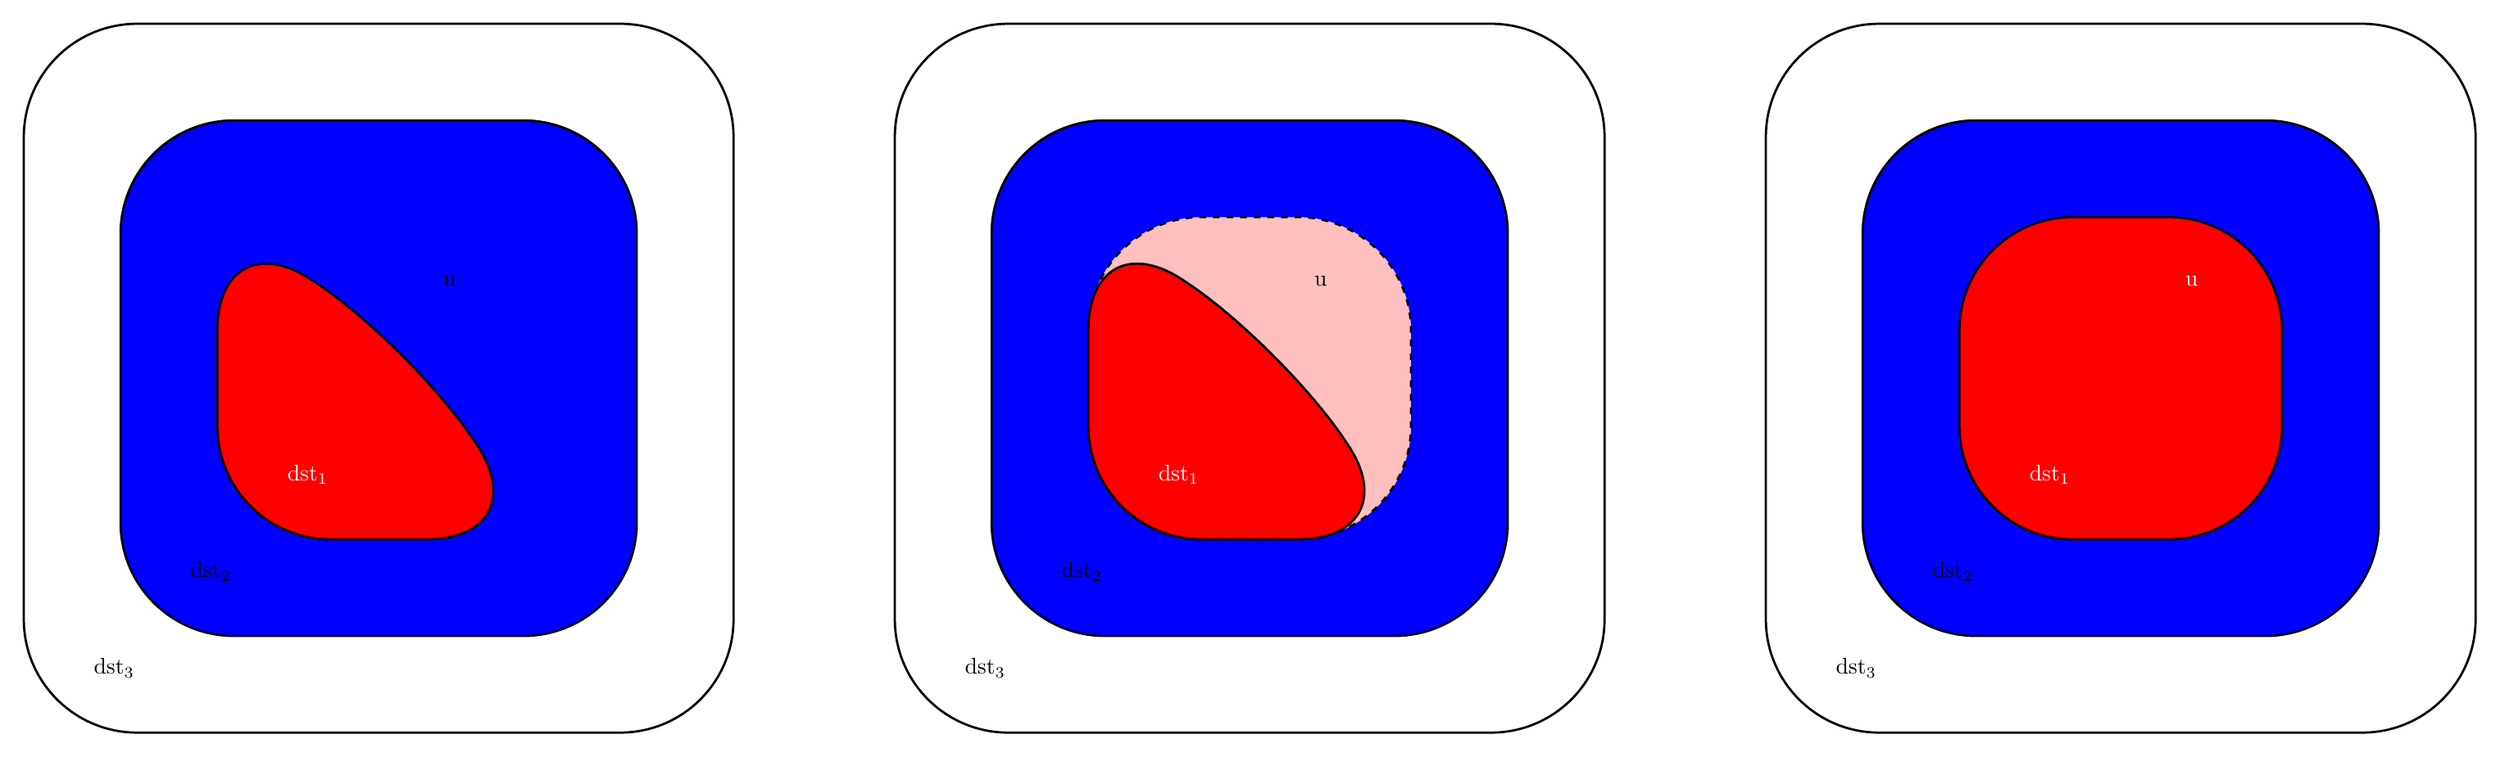
\begin{tikzpicture}[
  popped/.style={rounded corners=50pt, line width=1pt, draw, fill=red},
  fringe/.style={rounded corners=50pt, line width=1pt, draw, fill=blue},
  popping/.style={rounded corners=50pt, line width=1pt, draw, dashed, fill=pink},
  unseen/.style={rounded corners=50pt, line width=1pt, draw}]
  \draw[unseen] (0,0) -- (\s,0) -- (\s,\s) -- (0,\s) -- cycle;
  \draw[fringe] (1.5,1.5) -- (9.5,1.5) -- (9.5,9.5) -- (1.5,9.5) -- cycle;
  \draw[popped] (3,3) -- (8,3) -- (6,6) -- (3,8) -- cycle;
  \node at (1.4,1) {dst$_3$};   
  \node at (2.9,2.5) {dst$_2$};   
  \node at (4.4,4) {\color{white}dst$_1$}; 
  \node at (6.6,7) {u};
\tikzset{shift={(13.5,0)}}

  \draw[unseen] (0,0) -- (\s,0) -- (\s,\s) -- (0,\s) -- cycle;
  \draw[fringe] (1.5,1.5) -- (9.5,1.5) -- (9.5,9.5) -- (1.5,9.5) -- cycle;
  \draw[popping] (3,3) -- (8,3) -- (8,8) -- (3,8) -- cycle;
  \draw[popped] (3,3) -- (8,3) -- (6,6) -- (3,8) -- cycle;
  \node at (1.4,1) {dst$_3$};   
  \node at (2.9,2.5) {dst$_2$};   
  \node at (4.4,4) {\color{white}dst$_1$}; 
  \node at (6.6,7) {u};     

\tikzset{shift={(13.5,0)}}

  \draw[unseen] (0,0) -- (\s,0) -- (\s,\s) -- (0,\s) -- cycle;
  \draw[fringe] (1.5,1.5) -- (9.5,1.5) -- (9.5,9.5) -- (1.5,9.5) -- cycle;
  \draw[popped] (3,3) -- (8,3) -- (8,8) -- (3,8) -- cycle;
  \node at (1.4,1) {dst$_3$};   
  \node at (2.9,2.5) {dst$_2$};   
  \node at (4.4,4) {\color{white}dst$_1$}; 
  \node at (6.6,7) {\color{white}u};       
\end{tikzpicture}

}% end centering
\end{adjustbox}